\documentclass{article}
\usepackage[utf8]{inputenc}
\usepackage[T1]{fontenc}
\usepackage[french]{babel}
\usepackage{graphicx}
\usepackage{listings}
\usepackage{color}
\usepackage{geometry}
\usepackage{array}
\geometry{hmargin=2.5cm,vmargin=3cm}
\definecolor{dkgreen}{rgb}{0,0.6,0}
\definecolor{gray}{rgb}{0.5,0.5,0.5}
\definecolor{mauve}{rgb}{0.58,0,0.82}

\lstset{frame=tb,
  language=Java,
  aboveskip=3mm,
  belowskip=3mm,
  showstringspaces=false,
  columns=flexible,
  basicstyle={\small\ttfamily},
  numbers=none,
  numberstyle=\tiny\color{gray},
  keywordstyle=\color{blue},
  commentstyle=\color{dkgreen},
  stringstyle=\color{mauve},
  breaklines=true,
  breakatwhitespace=true,
  tabsize=3
}

\date{\today}
\author{Tarik Atlaoui \\ Nicolas Peugnet \\ Kimmeng Ly \\ Max Eliet}

\begin{document}


\begin{titlepage}
	\enlargethispage{2cm}
	\newcommand{\HRule}{\rule{\linewidth}{0.5mm}}
	\center
	\textsc{\LARGE
	Pre-rapport du PSAR 
	} \\[1cm]
	\HRule \\[0.4cm]
	{ \huge \bfseries API générique pour le développement d'applications réparties \\[0.15cm] }
	\HRule \\[4cm]
	\large{Tarik Atlaoui \\[3mm] Nicolas Peugnet \\[3mm] Kimmeng Ly \\[3mm] Max Eliet} \\[3cm]
	09 Mars 2020 \\[3cm]
	\hfill 
\includegraphics[width=5cm]{logoSU.jpg}
\end{titlepage}

	\newpage
	\pagenumbering{arabic}
		\section{Introduction}
			\subsection{Les applications réparties : qu'est-ce ?}
			\large{ Avant de commencer, il est important de définir ce qu’est une application répartie. Dans notre cas, nous pouvons voir une application répartie comme un ensemble d’entités logicielles, de composants qui peuvent être développés dans différents langages de programmation, s’exécutant sur plusieurs sites et qui sont reliés entre eux par une interface ou un réseau de communication.}
			\subsection{Les difficultés à programmer une application répartie}
			\large { Aujourd’hui la programmation d’applications réparties est devenue une réalité du monde informatique, cette forme de programmation permet d'augmenter la disponibilité des applications et de diminuer leur temps d'exécution. Cependant, réaliser une application répartie reste une tâche délicate. En effet, nous devons prendre en compte la maintenabilité et la réutilisabilité des programmes. De plus, les accès concurrents peuvent créer des erreurs et des sources d'incohérence. C’est pourquoi il est très important de montrer que ces programmes fonctionnent bien avec des tests unitaires tout en respectant le cahier des charges.}
		\section{Méthode de développement}
			\subsection{API réelle : avantages/inconvénients + exemple API(MPI ou autre)}
			%RESTE A COMPLETER ICI
			L'API de MPI est avant tout une norme pour le passage de messages entre différents ordinateurs ou au sein d'un même ordinateur.
			Elle est énormément utilisée pour la communication sur des architectures distribuées.
			Dans notre cas, elle s'est révélée extrêmement intéressante car MPI a été implémentée sur presque toutes les architectures ainsi elle 
			a été adaptée pour chacune de la façon la plus optimale. Cependant les tests et le debug sur celle-ci restent difficiles dû a l'impossibilité 
			d'avoir un contrôle sur les évenements qui apparaissent, contrairement à PeerSim.
			\newpage
			\subsection{API simulation à évenements discrets : qu'est-ce ? + avantages/inconvénients + exemple(PeerSim ou autre)}
				Qu'entend-on par \textit{simulation à événements discrets}? C'est une simulation dont le temps évolue seulement lorsqu'un événement survient sur un noeud, et donc de même l'état du système ne peut être modifié qu'à ces moments là.

				On distingue donc deux entités : les noeuds, et les événements qui sont caractérisés par une date de délivrance, un noeud destinataire, et des données.

				Les principaux avantages d'un tel type de simulation sont : son déterminisme et donc une capacité à reproduire des bugs, et une charge de calcul réduite aux événements qu'on décide de simuler. Toutefois, il faut savoir trouver un équilibre entre une simulation trop simpliste et une simulation trop précise ralentie par trop d'événements.

				Dans notre cas, nous nous sommes dirigés vers PeerSim comme simulateur à événements discrets, car il est codé en Java et possède une API relativement simple d'utilisation.

				PeerSim est utilisé pour créer des nœuds et simuler une architecture pair-à-pair en générant des protocoles et des événements qui sont définis par l'utilisateur. Une éxécution est toujours ce qui permet d'accélérer le débug d'une application répartie avant son déploiement ou de reproduire une séquence d'événements qui a provoqué un bug sur une application déja existante.

			\newpage
			\subsection{Aperçu de l'implémentation d'un anneau avec les deux API}
				{\bfseries Implémentation en MPI}
				\begin{lstlisting}
public class RingMpi {
	public static void main(String[] args) {
			MPI.Init(args);
			Comm comm = MPI.COMM_WORLD;
			int size = comm.getSize();
			int rank = comm.getRank();
			int neighbour = (rank + 1) % size;
			int hellotag = 1;
			Integer msg = 0;
			Status status;
			if (rank == 0) {
				comm.send(msg, 0, MPI.INT, neighbour, hellotag);
				status = comm.recv(msg, 0, MPI.INT, MPI.ANY_SOURCE, hellotag);
			} else {
				status = comm.recv(msg, 0, MPI.INT, MPI.ANY_SOURCE, hellotag);
				comm.send(msg, 0, MPI.INT, neighbour, hellotag);
			}
			System.out.println(rank + " Received hello from " + status.getSource());
			MPI.Finalize();
		}
	}
}
				\end{lstlisting}
				{\bfseries Implémentation en PeerSim}
				\begin{lstlisting}
public class HelloProtocol implements EDProtocol {
	//Declarations d'attributs et fonctions retirees pour la clarte du code
	...
	//Un noeud souhaite faire sa diffusion du message a son voisin
	public void direVoisin(Node host) {
		Transport tr= (Transport) host.getProtocol(pid_transport);
		Node dest=Network.get((int) ((host.getID()+1)%Network.size()));
		Message mess= new Message(host.getID(),(host.getID()+1)%Network.size(),my_pid, new ArrayList<>(myList));
		tr.send(host, dest, mess, my_pid);

		deja_dit_voisin=true;
	}

	//Traitement a effectuer lorsqu'on recoit un HelloMessage
	private void receiveHelloMessage(Node host, HelloMessage mess) {
		System.out.println("Noeud "+ host.getID() + " : a recu Hello de "+mess.getIdsrc()+ " sa liste = "+mess.getInfo());
		if(!deja_dit_voisin) {
			direVoisin(host);
		}
	}
}
				\end{lstlisting}
		\section{Motivation et objectif global}
			\subsection{API générique : avantages, modèle de programmation(ici événementiel)}
				Le but de notre projet est de produire une API générique sur un modèle de programmation événementielle afin de faciliter le développement de futures applications réparties, en permettant de s'abstraire du support d'éxécution au niveau du code métier. \par
Pouvoir éxécuter le même code métier aussi bien sur une plateforme réelle que sur un simulateur permet au développeur d'une application répartie de passer de l'un à l'autre, sans risquer d'en  modifier son comportement en adaptant le code. \newline Il peut donc profiter des avantages d'un simulateur, comme la vision globale du système et le déterminisme des séquences d'éxécution  sans crainte d'y introduire de nouveaux bugs. \par
 
			\newpage
			\subsection{Aperçu de l'implémentation d'un anneau avec l'API générique}
				\begin{lstlisting}
public class ExampleNodeProcess extends NodeProcess {

	public static class ExampleMessage extends Message{
	
		private static final long serialVersionUID = 1L;
		private String s;
		public ExampleMessage(int src, int dest, String s) {
			super(src, dest);
			this.s = s;
		}

		public String getS() {
			return s;
		}

	}

	@MessageHandler
	public void processExampleMessage(ExampleMessage message) {
		int host = infra.getId();
		System.out.printf("%d Received '%s' from %d\n", host, message.getS(), message.getIdsrc());
		if (host != 0) {
			int dest = (host + 1) % infra.size();
			infra.send(new ExampleMessage(infra.getId(), dest, "bonjour"));
		}
		infra.exit();
	}

	@Override
	public void start() {
		if (infra.getId() == 0) {
			infra.send(new ExampleMessage(infra.getId(), 1, "bonjour"));
		}
	}
}

public class BasicTest {

	@Test
	public void MpiExample() {
		Ppi.main(new String[] { ExampleNodeProcess.class.getName(), MpiRunner.class.getName() });
		assertTrue(true);
	}

	@Test
	public void PeersimExample() {
		Ppi.main(new String[] { ExampleNodeProcess.class.getName(), PeerSimRunner.class.getName() });
		assertTrue(true);
	}
}
				\end{lstlisting}
		\section{Les étapes de réalisation}
			\subsection{Définition API générique}
			\hspace*{-2cm} 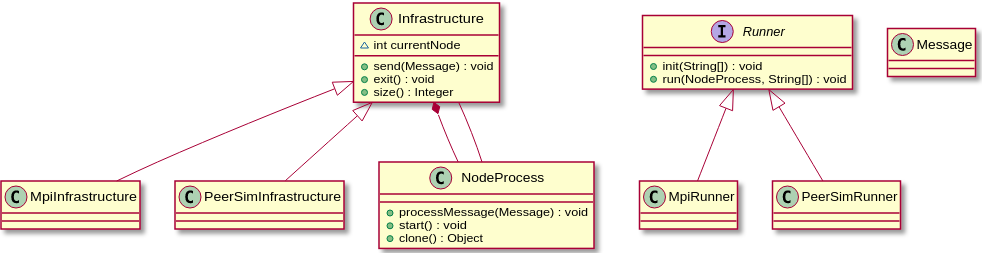
\includegraphics[width=19cm]{Ppi_uml.png}
			Nous avons commencé par définir une classe abstraite Infrastructure  qui contient tous les éléments qui doivent être implantés par les deux API.
			\newline
			Sachant que le lancement des deux applications est radicalement différent, nous avons réalisé qu'il était primordial que les deux 
			lancements soient unifiés pour permettre un développement plus rapide et sûr, pour y remédier nous avons créé l'interface Runner qui nous permet 
			d'instancier des exécutions des deux API avec les mêmes arguments, ainsi il suffit d'instancier MPIRunner ou PeerSimRunner avec en argument
			le nom de la classe qui implante NodeProcess, le nom du runner et le nombre de processus.
			\subsection{Définitions des primitives offertes et explication}
			\begin{lstlisting}
			public void start();
			\end{lstlisting}
			La primitive start  doit etre redéfinie par l'utilisateur et permet de définir le code à éxécuter par le processus lors de son lancement.
			\begin{lstlisting}
			public void processMessage(Message message);
			\end{lstlisting}
			De même pour processMessage qui permet  de définir le comportement du processus lors de la réception d'un message.
			\begin{lstlisting}
			abstract class Message implements Serializable
			\end{lstlisting}
			Message est la classe définie afin de permettre une abstraction du traitement des messages et doit etre étendue par l'utilisateur.

			\begin{lstlisting}
				public class Ppi
				//utilisation
				Ppi.main(new String[] {NodeProcess.class.getName(),Runner.class.getName()});
			\end{lstlisting}
			La class Ppi est le main de notre application, elle permet d'executer le code utilisateur en MPI ou en PeerSim.

			\subsection{Implantation vers MPI}
			Pour l'implantation de l'adapteur permettant d'utiliser MPI nous avons commencé par implanter un algorithme simple en utilisant cette dernière.
			Une fois que nous avions compris comment MPI fonctionnait nous avons étendu la class Infranstructure qui représente l'abstraction des deux adapteurs implantés, pour MPI la class MpiInfrastructure nous permet de communiquer avec MPI en ajoutant  une couche sur les primitives de MPI.
			Nous avons, cependant, dû ajouter une boucle  afin d'adapter le fonctionnement de MPI à celui de PeerSim.
			\subsection{Implantation vers PeerSim}
			Dans le cas de PeerSim, l'implantation de notre API consistait principalement à effectuer un Adapter avec l'API déjà existante de PeerSim, et donc la part la plus importante du travail était de comprendre le fonctionnement des quelques classes de PeerSim nécessaires pour faire le lien entre les deux API. Il a aussi fallu adapter certaines de nos classes pour PeerSim, par exemple rendre notre NodeProcess clonable. 
			\subsection{API pour un scenario}
			L'utilisateur aura aussi accès à une API permettant de décrire un scenario où il devra spécifier en premier lieu
			le nombre de noeuds demandé, puis préciser sur quelle API le scénario devra être exécuté, et enfin les événements et leur date qui devront être appelés.
			Sachant que MPI travaille sur de vraies machine et que le temps d'arrivée des messages est inconnu, on ne promet pas l'éxécution exacte du scénario demandé.
			\newline
			\newline
			A fin de demandé l'éxecution d'un scénario il faut aussi étandre la class NodeProcess et y 
			implanter les fonctions qui fon office de events , et dont on peux programmer l'appel avec delais données.
			Pour le faire il faut un fichier au format Json avec le format suivant.
			\subsection{Format}
			\begin{lstlisting}
				{"Off":[{
					"node":0,
					"start":100
					}],
				"events":[{
					"args":[{"val":"MonArgument1","type":"String"},{"val":4,"type":"Integer"}]
					"FunctionName":"End",
					"Node":1,
					"Delay":900},
					{{
						"args": [],
						"FunctionName": "doSomething",
						"Node": 2,
						"Delay": 300
					}],
					"On":[ { "node":0, "start":10000}]}
			\end{lstlisting}
			Les Json object nomé "off","on" et "events" fon office de conteuneur pour les différent appelés demander,
			chaqu'un contient une liste des evenement,par exemple {\color{magenta} "off"} sa liste contien un sous objet qui définis
			\newline
			{\color{magenta} "node"} qui indique le noeud sur le quelle a la date {\color{magenta} "start"} le noeud va arreter de répondre au message
			l'inverse {\color{magenta} "On"} réactive le noeud et permette a eux deux de simuler une panne.
			\newline
			\newline
			l'objet {\color{magenta} "events"} représente l'appel d'une fonction utilisateur l'element {\color{magenta} "args"} représente les argument de la fonction 
			doit etre données dans le meme ordre que ce de la fonction et spécifier le type de chaque arguments ainsi que ça valeur.
			\newline
			Notons que les type des arguments accepter sont les type de base de java.
			Enfin la clé {\color{magenta} "FunctionName"} représente le nom de la fonction a appeler.
			\newline
			\newline
			Pour aider la construction du fichier de configuration nous proposont les primitive de la class ProtocolTools suivante:
			\newline
			Pour construire un appelle de fonction
			\begin{lstlisting}
				public static JSONObject eventBuilder(String funcName , int node, long delay, List<Object> args);
			\end{lstlisting}
			Pour construire un appelle de fonction
			\begin{lstlisting}
				public static JSONObject StateBuilder(int node, long start_at);
			\end{lstlisting}

			Enfin pour lancée l'execution du scénario il faut juste ajouter le nombre de processus et le chemin ver le fichier Json au runneur souhaiter.

			%\subsection{Rédaction du rapport}

		\section{Plan de validation}
		\subsection{Tests de validation}
		Pour chaque fonctionnalité ajoutée nous ajoutons un test et nous nous assurons que les tests précédents fonctionnent toujours.
		\newline
		La classe BasicTest est la toute première classe de tests que nous avons implémenté, elle s'assure que les fonctionnalités de base de notre API
		send/receive et le format de description de scénario restent fonctionnels malgré les nouveaux ajouts.

		Plusieurs algorithmes distribués seront implantés et testé unitairement dont celui de l'anneau et au moins une exclusion mutuelle.
		%Comment montrer que cela fonctionne bien, tests unitaires, respect du cahier des charges
		\subsection{Démonstration}
		Lors de la soutenance, une démonstration sera lancée pour montrer de façon évidente que notre interface fonctionne.
		Le même code applicatif sera executé sur plusieurs machines (potentiellement virtuelles) une première fois via l'infrastructure MPI puis sur celle de Peersim.
		pour prouver le bon fonctionnement de notre application nous avons décidé de faire jouer une note musicale aux ordinateurs où chacun devra attendre un certain délai 
		avant de jouer sa note tout en s'assurant qu'il est le seul à jouer à ce moments pour mpi et pour PeerSim nous allons nous assurer que l'exécution est déterministe
		\section{Planning des tâches}
			\subsection{Une deadline pour chaque tâche dans un ordre chronologique}
			\begin{tabular}{|c|c|}
				\hline
				Tâche & Date d'échéance \\[1mm]
				\hline
				Se familiariser avec MPI et Peersim & 17/02 \\[1mm]
				\hline
				Proposer une API générique & 24/02 \\[1mm]
				\hline
				Implanter l'API pour MPI et pour PeerSim & 02/03 \\[1mm]
				\hline
				Créer une classe abstraite Message & 09/03 \\[1mm]
				\hline
				Unifier le lancement de l'application & 09/03 \\[1mm]
				\hline
				Rédiger le carnet de bord & 16/03 \\[1mm]
				\hline
				Rédiger le pre-rapport & 23/03 \\[1mm]
				\hline 
				Implanter l'aiguillage automatique des messages & 23/03 \\[1mm]
				\hline
				Ajouter la fonctionnalité de description de scenario & 30/03 \\[1mm]
				\hline
				Ajouter des fonctionnalités de wait/notify & 20/04 \\[1mm]
				\hline 
				Rédiger le rapport final & 27/04 \\[1mm]
				\hline
				Soutenance finale & XX/05 \\[1mm]
				\hline
			\end{tabular}
\end{document}
